\section{Results}

\subsection{Multi-wavelength single-molecule co-localization (CoSMoS) methods}

We aim to improve methods for elucidating the molecular mechanisms of biochemical processes \textit{in vitro} using multi-wavelength single-molecule fluorescence colocalization microscopy. The key features of a CoSMoS experiment include: 1) One species of fluorescently labeled molecule (called the “target”) is tethered to the surface. Targets are immobilized at a surface density sufficiently low that the mean nearest-neighbor distance is large relative to the point-spread function (i.e., the diffraction-limited spot size) of the microscope.
2) Molecules, each species labeled with a different dye color, are added to the solution over the surface, typically at concentrations < 1 $\mu$M. When these “binder” molecules are freely diffusing in solution, they are invisible in TIRF. In contrast, when they are bound to the target, single binder molecules are detected as discrete fluorescent spots (Figure \ref{fig:cosmos_experiment}). The combination of features 1 and 2 means that formation of an individual binder-target complex is detected as spot appearance; dissociation of a binder-target complex is detected as spot disappearance \citep{Friedman2006-kb, Friedman2015-nx}.

The CoSMoS data set consists of a set of images where we have $N$ target sites ($n \in \{1,\dots,N\}$) each consisting of a series of $F$ different images in a recording ($f \in \{1,\dots,F\}$) (a “recording”). Each image is represented as a matrix (2D-array) of $P \times P$ pixel intensities ($i,j \in \{1,\dots,P\}$). We denote entire data set as a multi-dimensional array $D$ with the shape $N \times F \times P \times P$ where the value of a specific pixel intensity can be obtained by indexing as $D_{nfij}$. 

\begin{figure}
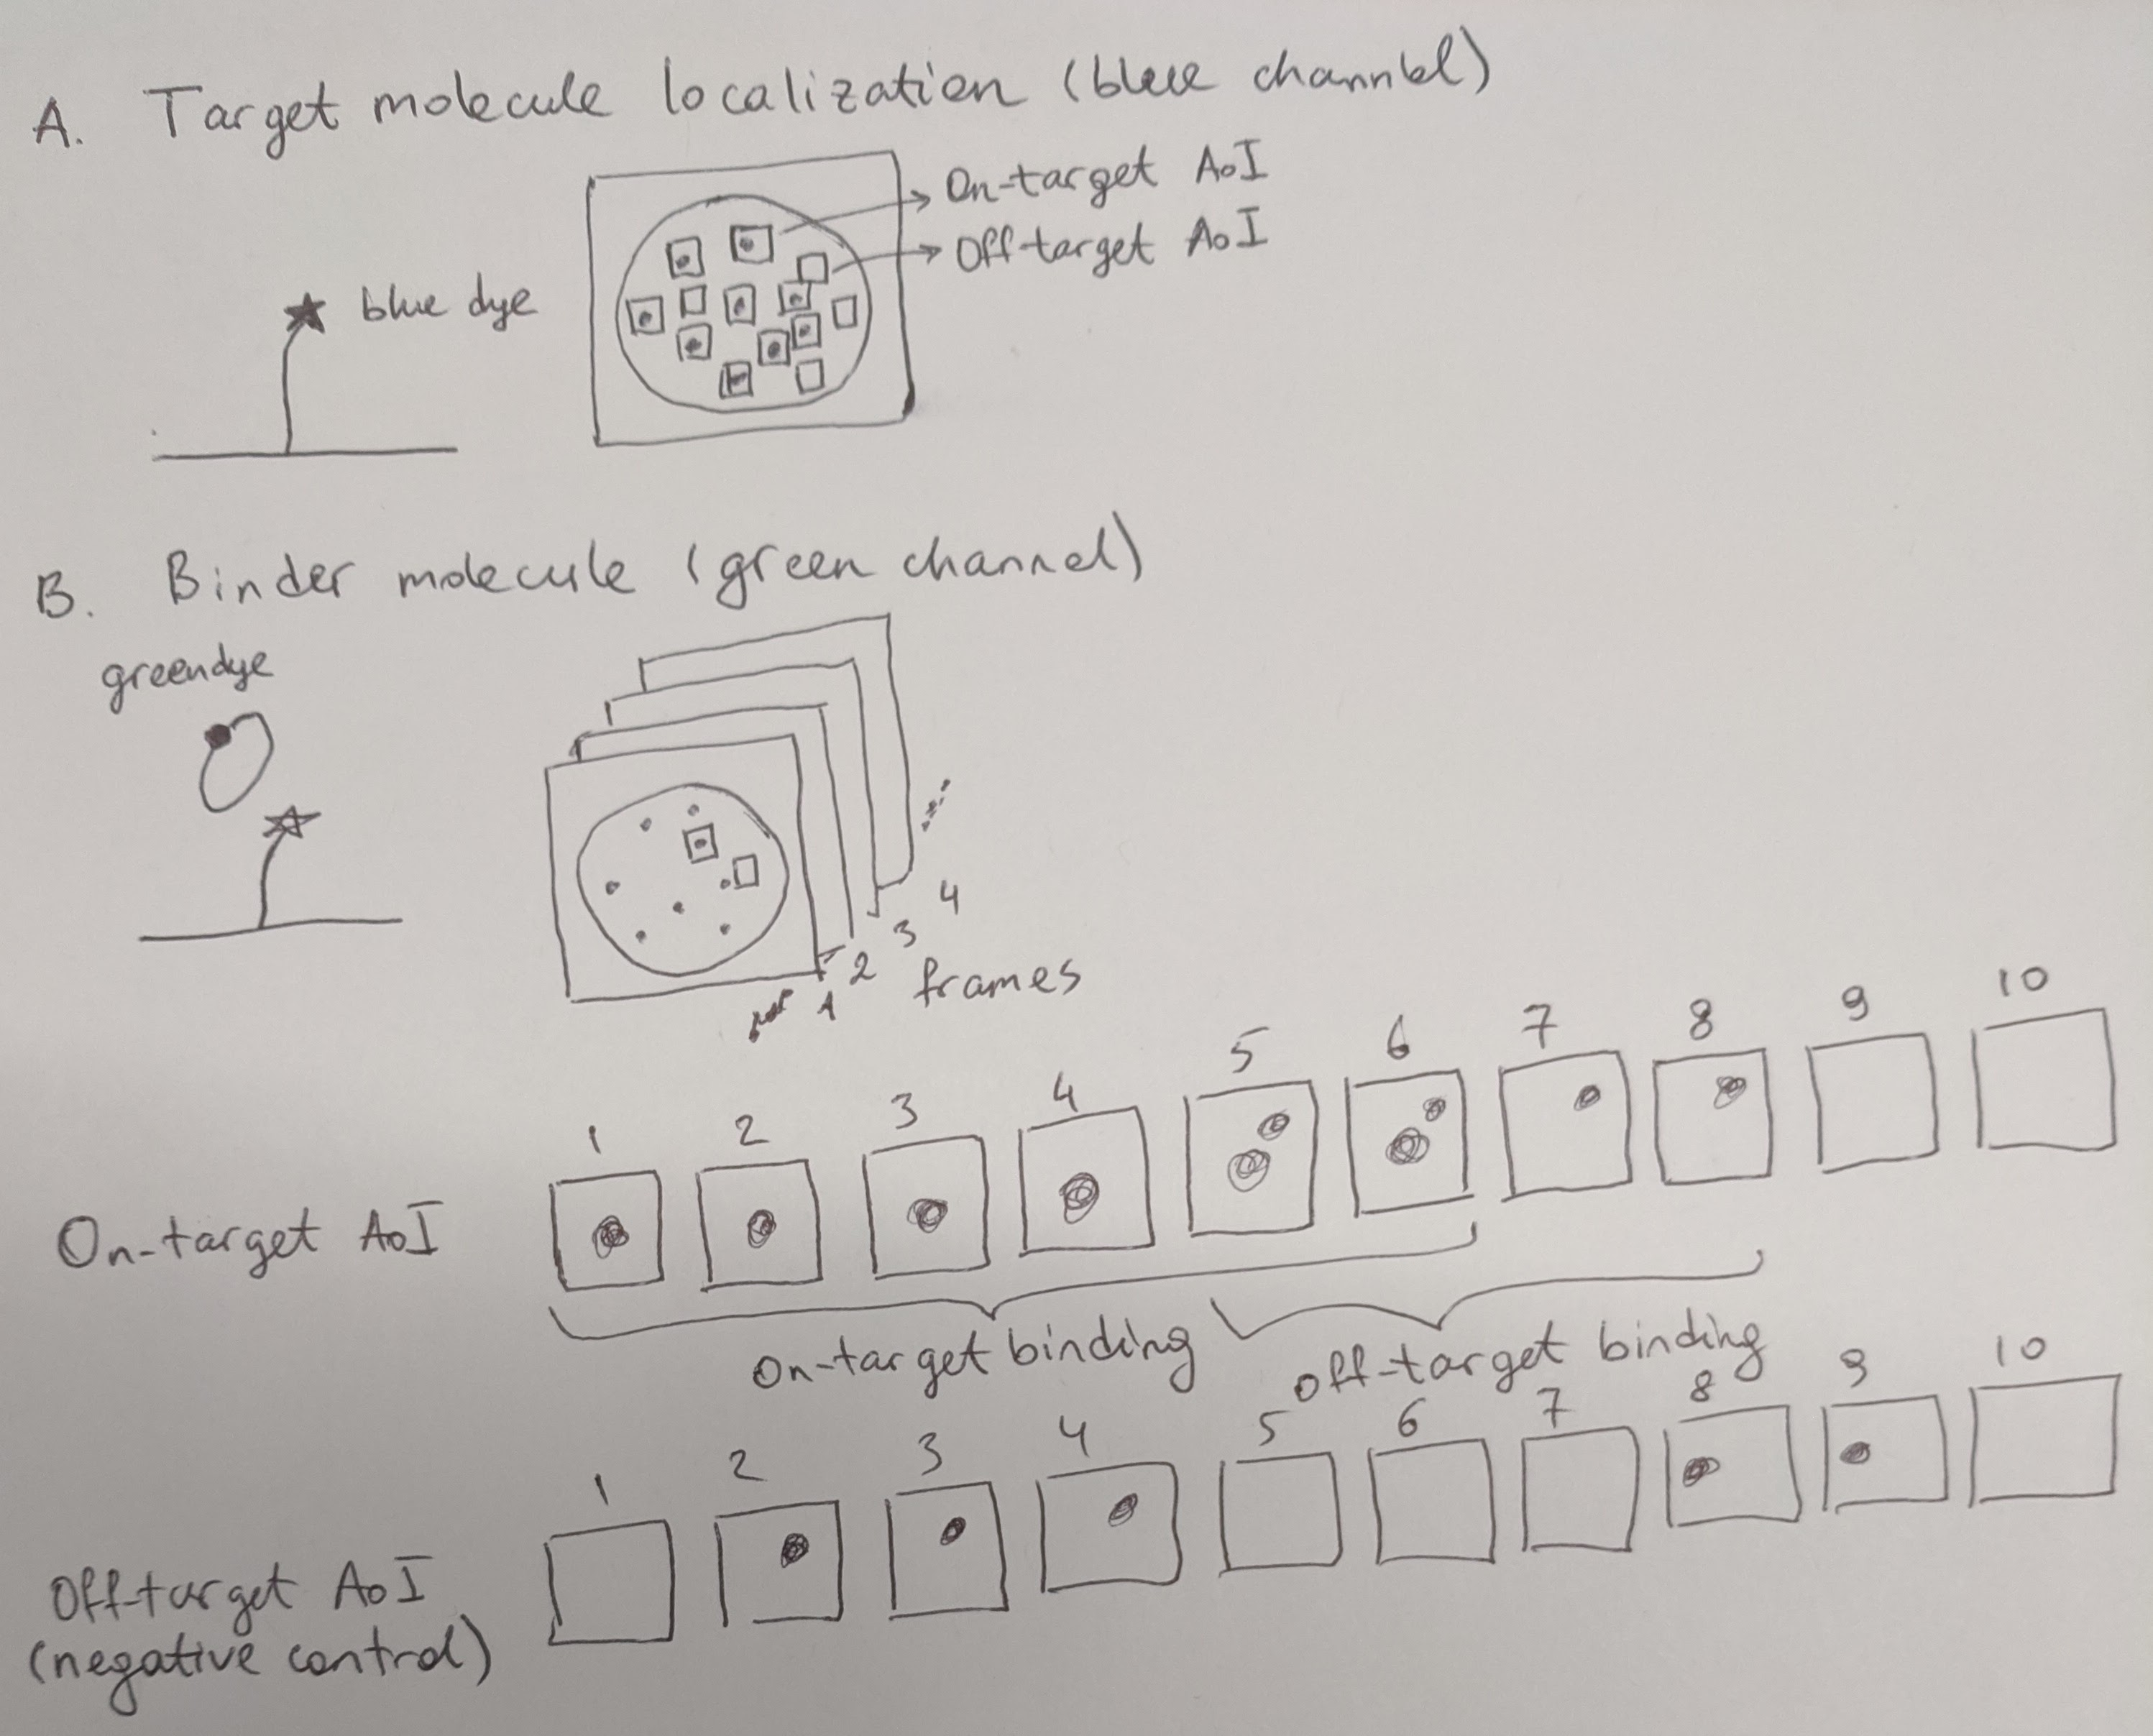
\includegraphics[width=\linewidth]{figures/figure1.jpg}
\caption{Co-localization single molecule spectroscopy experiment. (A) Target molecules are localized in the blue channel and then on-target and off-target areas of interest are selected. (B) Movies of the binder molecule collected in the green channel. In selected AoI binder molecules can be on-target, off-target, or absent.}
\label{fig:cosmos_experiment}
%% If the optional argument in the square brackets is "none", then the caption *will not appear in the main figure at all* and only the full caption will appear under the supplementary figure at the end of the manuscript.
%\figsupp[Shorter caption for main text.]{This is a supplementary figure's full caption, which will be used at the end of the manuscript.}{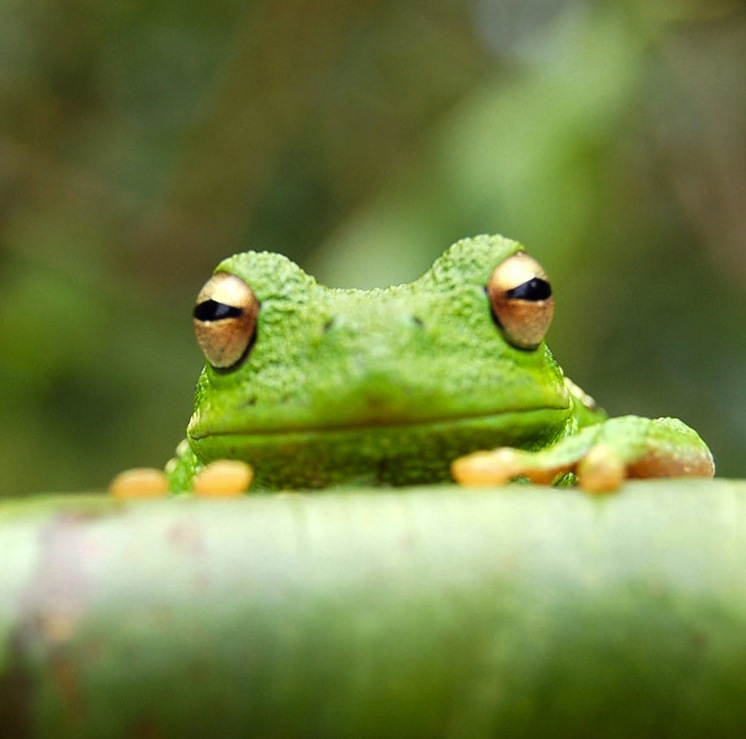
\includegraphics[width=6cm]{frog}}\label{figsupp:sf1}
%\figsupp{This is another supplementary figure.}{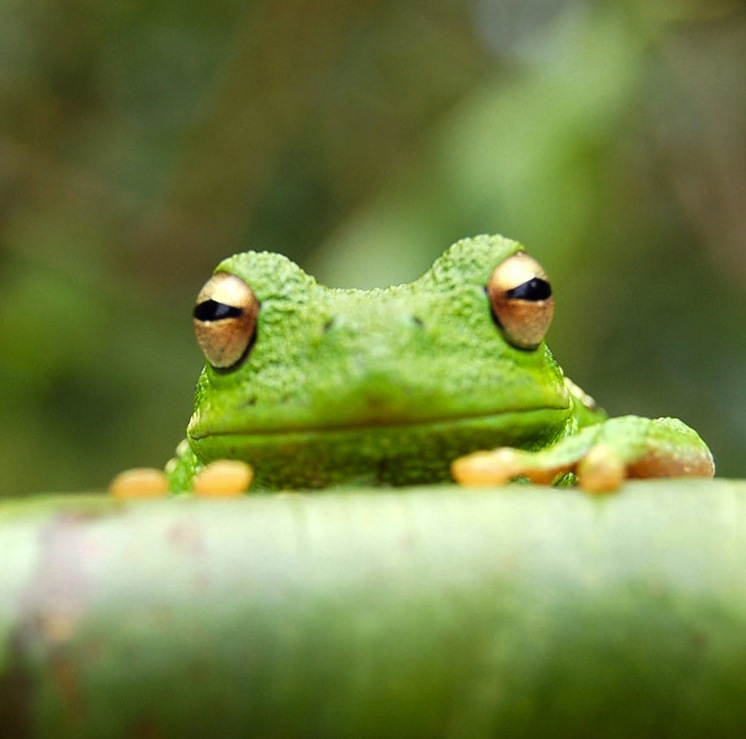
\includegraphics[width=6cm]{frog}}
%\figdata{This is a description of a data source.}\label{figdata:first}
%\figdata{This is another description of a data source.}\label{figdata:second}
\end{figure}

\subsection{Approach}

\subsubsection{Image model}

Distinctive feature of our approach is that we directly model 2D images at target sites which has not been previously done to our knowledge. CoSMoS images consist of background intensity and diffraction-limited spots. Local background intensity of the image is parameterized by scalar $b_{nf}$. We model the fluorescence spot as a 2D Gaussian which accurately approximates fluorescence microscope point spread function \citep{Zhang2007-rb}. Our model assumes that at maximum $K$ number of spots can be present in a single image. Each individual spot ($k \in \{1,\dots,K\}$) is parameterized by existence indicator ($m_{knf} \in \{0,1\}$), integrated spot intensity ($h_{knf}$), spot width ($w_{knf}$), and position relative to the target ($x_{knf},y_{knf}$). When the spot is absent ($m_{knf}=0$) the intensity is at the baseline level. The ideal shape of the image ($\mu^D_{nf}$) is calculated as the sum of the background intensity and 2D Gaussian spots present in the image. Figure shows ideal image shapes for cases when there are no spots (A), one spot (B), and two spots (C). Finally, each image has an index variable for the on-target spot ($\theta_{nf} \in \{0,1,\dots,K\}$) where zero means that the on-target spot is absent.

\subsubsection{Noise model}

Scatter about the expected value of pixel intensity ($\mu^D_{nfij}$) is determined by photonic shot noise and the gain of the camera. Shot noise originates from a stochastic nature of photon counting which can be modeled by a Poisson process. Thus, the number of photons that fall on each pixel of the camera is Poisson distributed where variance of the signal equals the mean value. Gain is the camera setting that amplifies the signal from camera sensors. Our model uses Gamma distribution parameterized by mean intensity ($\mu^D_{nfij}$) and gain ($g$) to model the linear relationship between the expected value of the signal and the variance with which the signal scatter about its expected value. Figure shows images  where the ideal images were perturbed with Gamma noise as described above.

\subsubsection{Spot detection}

Current spot detection methods produce binary outputs by using a bandpass-filter set by a user-specified intensity threshold \citep{Friedman2015-nx, Smith2019-yb}. To analyze the spot detection problem within the Bayesian framework we model spot intensities ($h_{knf}$) as a mixture of distribution of two classes with the hidden variable $m_{knf}$ specifying the identity of the class: a) no-spot baseline intensity distribution when $m_{knf}=0$ and b) spot intensity distribution of a binder molecule when $m_{knf}=1$.  This criterion ensures that fluctuations in background fluorescence are not
recognized as binding events. Unlike previous methods, this approach assigns probabilities of belonging to each class.

\subsubsection{Co-localization detection}

We employ the similar approach to detect co-localization and model the center of the spot to be distributed according to a mixture of two distributions. Non-specific binding can occur anywhere within the image and thus have a uniform distribution across the AoI image. On the other hand, co-localized spot denoted by an index variable $\theta_{nf}$ is scattered around target location within the co-localization accuracy which is modeled by distribution centered on target and standard deviation equal to the co-localization accuracy. For detected spots co-localization detection determines probabilities of being on-target or off-target binding. This is especially important for images where the precision of estimation of the center of mass quickly deteriorates with the low SNR. This ensures that ... It is important to note that spot detection and co-localization are part of a single unified model, rather than separate steps of the analysis.

Figure 3

\begin{figure}[ht]
  \begin{center}
    % model_pca2.tex
%
% Copyright (C) 2010,2011 Laura Dietz
% Copyright (C) 2012 Jaakko Luttinen
%
% The MIT License
%
% See LICENSE file for more details.

% PCA model

%\beginpgfgraphicnamed{model-pca}
\begin{tikzpicture}

  % Define nodes

  % Y
  \node[obs]          (D)   {$D$}; %

  % W and X
  \node[det, above=of D]            (md) {$\mu^D$} ; % 
  \node[latent, above=of md] (w)   {$w$}; %
  \node[latent, above=of md, left=of w]  (h)   {$h$}; %
  \node[latent, above=of md, left=of h]  (b)   {$b$}; %
  \node[latent, above=of md, right=of w]  (x)   {$x$}; %
  \node[latent, above=of md, right=of x] (y)   {$y$}; %

  % b hyperparameters
  \node[const, above=2.8 of b, xshift=-0.5cm] (mb) {$\mu^b$} ; %
  \node[const, above=3.5 of b, xshift=0.5cm]  (bb) {$\beta^b$} ; %

  % h hyperparameters
  \node[const, above=3.5 of h, xshift=-0.5cm] (mh) {$\mu^h$} ; %
  \node[const, above=3.5 of h, xshift=0.5cm]  (bh) {$\beta^h$} ; %

  % w hyperparameters
  \node[const, above=3.5 of w, xshift=-0.5cm] (mw) {$\mu^w$} ; %
  \node[const, above=3.5 of w, xshift=0.5cm]  (nw) {$\nu^w$} ; %

  % xy hyperparameters
  \node[const, above=3.5 of x, xshift=-0.1cm] (mxy) {$\mu^{x,y}=0$} ; %
  \node[const, above=3.5 of y, xshift=0.1cm] (pr) {$\nu_{flat},\nu_{prox}$} ; %
  \node[det, above=1.4 of y]  (nxy) {$\nu^{x,y}$} ; %

  % Factors
  \factor[above=of D] {D-f} {left:$\mathcal{G}$} {} {} ; %
  \factor[above=0.6 of b] {b-f} {left:$\mathcal{G}$} {mb,bb} {b} ; %
  \factor[above=0.6 of h] {h-f} {left:$\mathcal{G}$} {mh,bh} {h} ; %
  \factor[above=0.6 of w] {w-f} {left:$\mathcal{B}$} {mw,nw} {w} ; %
  \factor[above=0.6 of x] {x-f} {left:$\mathcal{B}$} {mxy,nxy} {x} ; %
  \factor[above=0.6 of y] {y-f} {left:$\mathcal{B}$} {mxy,nxy} {y} ; %

  % D hyperparameters
  \node[const, right=8 of D-f] (g) {gain} ; %

  % m and theta
  \node[latent, right=of y-f] (m)   {$m$}; %
  \node[latent, above=0.5 of m] (t)   {$\theta$}; %

  % m and theta hyperparameters
  \node[det, right=1. of m]        (pm) {$\pi^m$} ; %
  \node[det, right=1. of t]        (pt) {$\pi^\theta$} ; %
  \node[const, right=of pt] (pz) {$\pi^z$} ; %
  \node[const, right=of pm] (lj) {$\lambda^j$} ; %

  % theta hyperparameters
  %\node[const, right=1.2 of t] (pt) {$\pi^\theta(\pi^z,\lambda^j)$} ; %

  % noise
  %\node[latent, right=2.5cm of y-f]         (t)   {$\tau$}; %
  %\node[const, above=of t, xshift=-0.5cm] (at)  {$\alpha_\tau$} ; %
  %\node[const, above=of t, xshift=0.5cm]  (bt)  {$\beta_\tau$} ; %

  % Factors
  \factor[right=of m] {m-f} {above:$\mathcal{C}$} {pm} {m} ; %
  \factor[right=of t] {t-f} {above:$\mathcal{C}$} {pt} {t} ; %
  %\factor[above=of x] {x-f} {left:$\mathcal{N}$} {mx,ax} {x} ; %
  %\factor[above=of t] {t-f} {left:$\mathcal{G}$} {at,bt} {t} ; %
  %\factoredge {dot,t} {y-f} {y} ; %

  \gate {m-gate} {(h-f)(h-f-caption)(h-f)(h-f-caption)(w-f)(w-f-caption)(x-f)(x-f-caption)(y-f)(y-f-caption)} {m}

  % Connect w and x to the dot node
  \factoredge[-] {g,md} {D-f} {D} ;
  \edge[-] {b,h,w,x,y} {md} ;
  \edge[-] {pz} {pt} ;
  \edge[-] {lj,t} {pm} ;
  \edge[-] {t,pr} {nxy} ;

  % Plates
  \plate {K} { %
    (h)(h-f)(h-f-caption) %
    (w)(w-f)(w-f-caption) %
    (x)(x-f)(x-f-caption) %
    (y)(y-f)(y-f-caption) %
    (m-gate) %
    (nxy)
  } {$\forall k \in \{ 1..K \}$} ;
  \plate {F} { %
    (K)
    (t)(t-f)(t-f-caption)(pt) %
    (m)(m-f)(m-f-caption)(pm) %
    (b)(b-f)(b-f-caption) %
    (md) %
    (D)(D-f)(D-f-caption) %
  } {$\forall f \in \{ 1..F \}$} ;
  \plate {N} { %
    (F)
    (mb)
  } {$\forall n \in \{ 1..N \}$} ;
  %\plate {} {%
    %(y)(y-f)(y-f-caption) %
    %(w)(w-f)(w-f-caption) %
    %(dot) %
    %(yx.north west)(yx.south west) %
  %} {$M$} ;

\end{tikzpicture}
%\endpgfgraphicnamed

%%% Local Variables: 
%%% mode: tex-pdf
%%% TeX-master: "example"
%%% End: 


  \end{center}
  \caption{Graphical model for the Bayesian classification model used in Pyro. The model has a modular structure consisting of three parts: classifier, the spot model, and the noise model. Hidden variables (circles) - background intensity ($b$), integrated intensity of the spot ($h$), width of the spot ($w$), position of the spot on the $x$-axis ($x$) and on the $y$-axis ($y$), existence indicator of spots ($m$), and index of the on-target spot ($\theta$). Observed variable (shaded circle) - image of the area of interest ($D$). Variables nested in plates are repeated for a number of times displayed at the bottom-right corner - target sites ($N$), frame count ($F$), number of spots in a single image ($K$). Densities are depicted as  small filled boxes. Deterministic functions are depicted as diamonds. Constants and hyperparameters are written without any borders. Gate (dashed box) represents variable activation conditioned on another variable.}
  \label{fig:graph}
\end{figure}

\begin{figure}
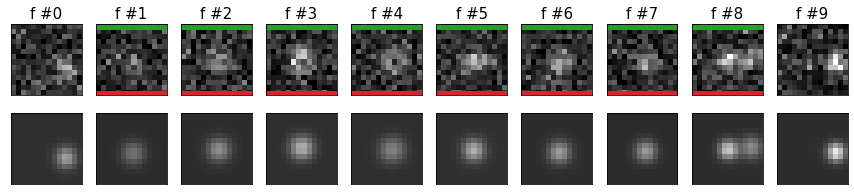
\includegraphics[width=\linewidth]{figures/figure2a.png}
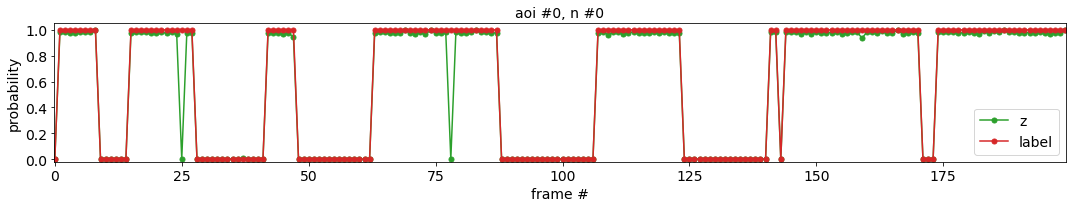
\includegraphics[width=\linewidth]{figures/figure2b.png}
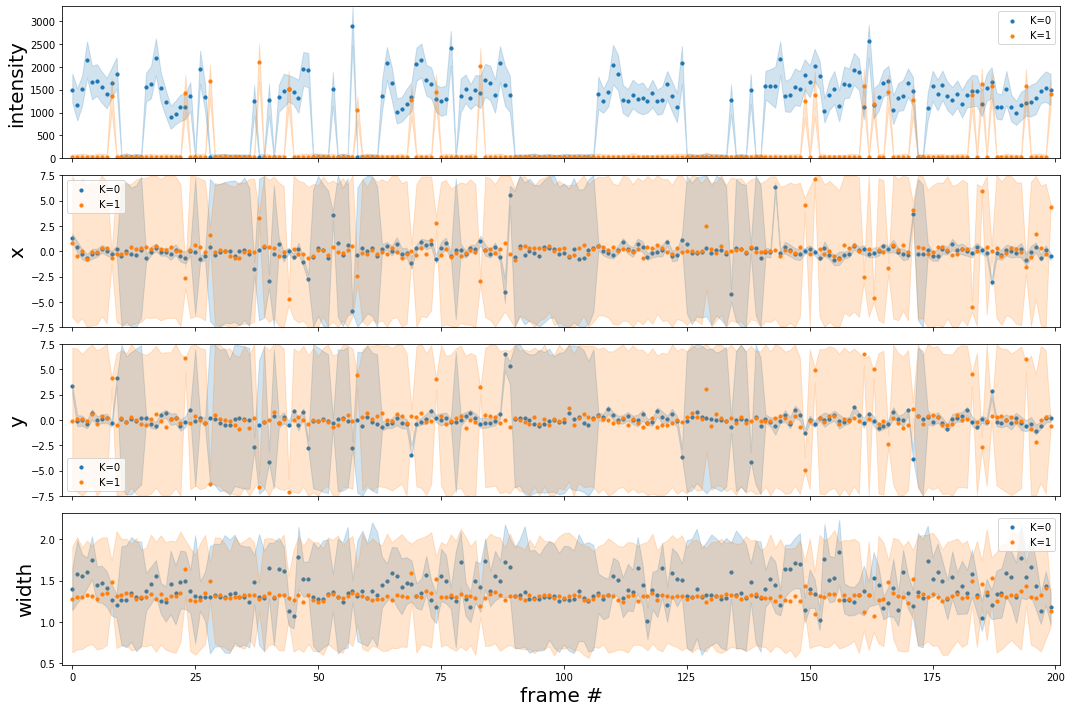
\includegraphics[width=\linewidth]{figures/figure2c.png}
\caption{Co-localization single molecule spectroscopy experiment. (A) Target molecules are localized in the blue channel and then on-target and off-target areas of interest are selected. (B) Movies of the binder molecule collected in the green channel. In selected AoI binder molecules can be on-target, off-target, or absent.}
\label{fig:view}
\end{figure}

\subsection{Comparison of Bayesian method with heuristic spot thresholding}

We have done two types of performance comparison between the Bayesian method and the heuristic spot thresholding method.

\subsubsection{Experimental data}

For the first performance comparison, images from real (i.e., not simulated) experimental data recordings were analyzed. In this experiment, we labeled the NusG protein with an orange dye. We then tethered to a microscope slide blue-dye-labeled DNA molecules at very low surface density (so that each molecule is resolved as a separate fluorescent spot) and observed real-time binding and dissociation of the other labeled molecules during the transcription process and its regulation. The signal from the orange dye was split between short wavelength and long wavelength channels. The signal in the short wavelength channel was attenuated to varying degree to produce data sets with a range of SNR. Images from the long wavelength channel with high SNR were analyzed to determine "true" identities of the images.

Each data set was analyzed by both the Bayesian method and the heuristic spot thresholding algorithm (Figure \ref{fig:real_data}). By comparison with the known “true” identities of the images, the accuracy of the resulting classifications was judged using a variety of specialized statistics for binary classification data, including true and false positive rates, true and false negative rates, and the Matthews Correlation Coefficient (MCC) \citep{Fawcett2006-bq, Matthews1975-rw}. The MCC statistic is widely regarded as a single overall, balanced measure which is meaningful even when the classes are of very different sizes. The MCC corresponds to the Pearson correlation coefficient between the estimated and “true” binary classifications. MCC=+1 represents a perfect prediction, MCC=0 a perfectly random prediction, and MCC=-1 indicates maximal disagreement between truth and estimation. Over a range of S/N, the Bayesian method gave image classification accuracy (as quantified by the MCC) better than the heuristic spot thresholding algorithm. 

\begin{figure}
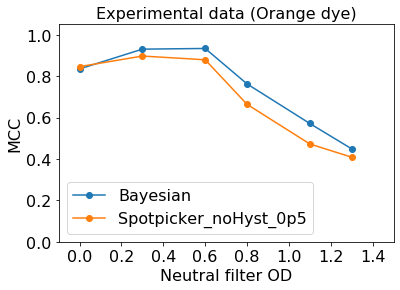
\includegraphics[width=\linewidth]{figures/figure4.png}
\caption{Performance comparison of the Bayesian method with the heuristic spot thresholding algorithm on real experimental data.}
\label{fig:real_data}
\end{figure}

\subsubsection{Simulated data}

In a second comparison, a series of simulated data sets were constructed for a range of signal-to-noise values. For each S/N, a set of 7,500 images (15 AoIs, 500 frames) of 14 by 14 pixels shape were generated using our probabilistic generative model. Each image is a combination of the background intensity plus randomly sampled 2-D Gaussian spots bound at the target and off-target with the intensity noise generated according to Gamma distribution.

Comparison of two methods showed similar performance on simulated data (Figure \ref{fig:simulated_data}). Taken together, these data demonstrated that the Bayesian method performs as well as the best existing CoSMoS data analysis method. Furthermore, Bayesian method achieves this performance automatically, with no adjustable parameters whatsoever, unlike the heuristic spot picker which attains this level of performance only after careful subjective trial-and-error manual adjustment of its three threshold parameters, a process that must be repeated tediously for each data set analyzed. Finally, our new Bayesian method produces a spot probability estimate for each image (not merely a Boolean spot/no spot determination) that can be used to inform subsequent kinetics calculations based on the results (e.g., the HMM analysis).

\begin{figure}
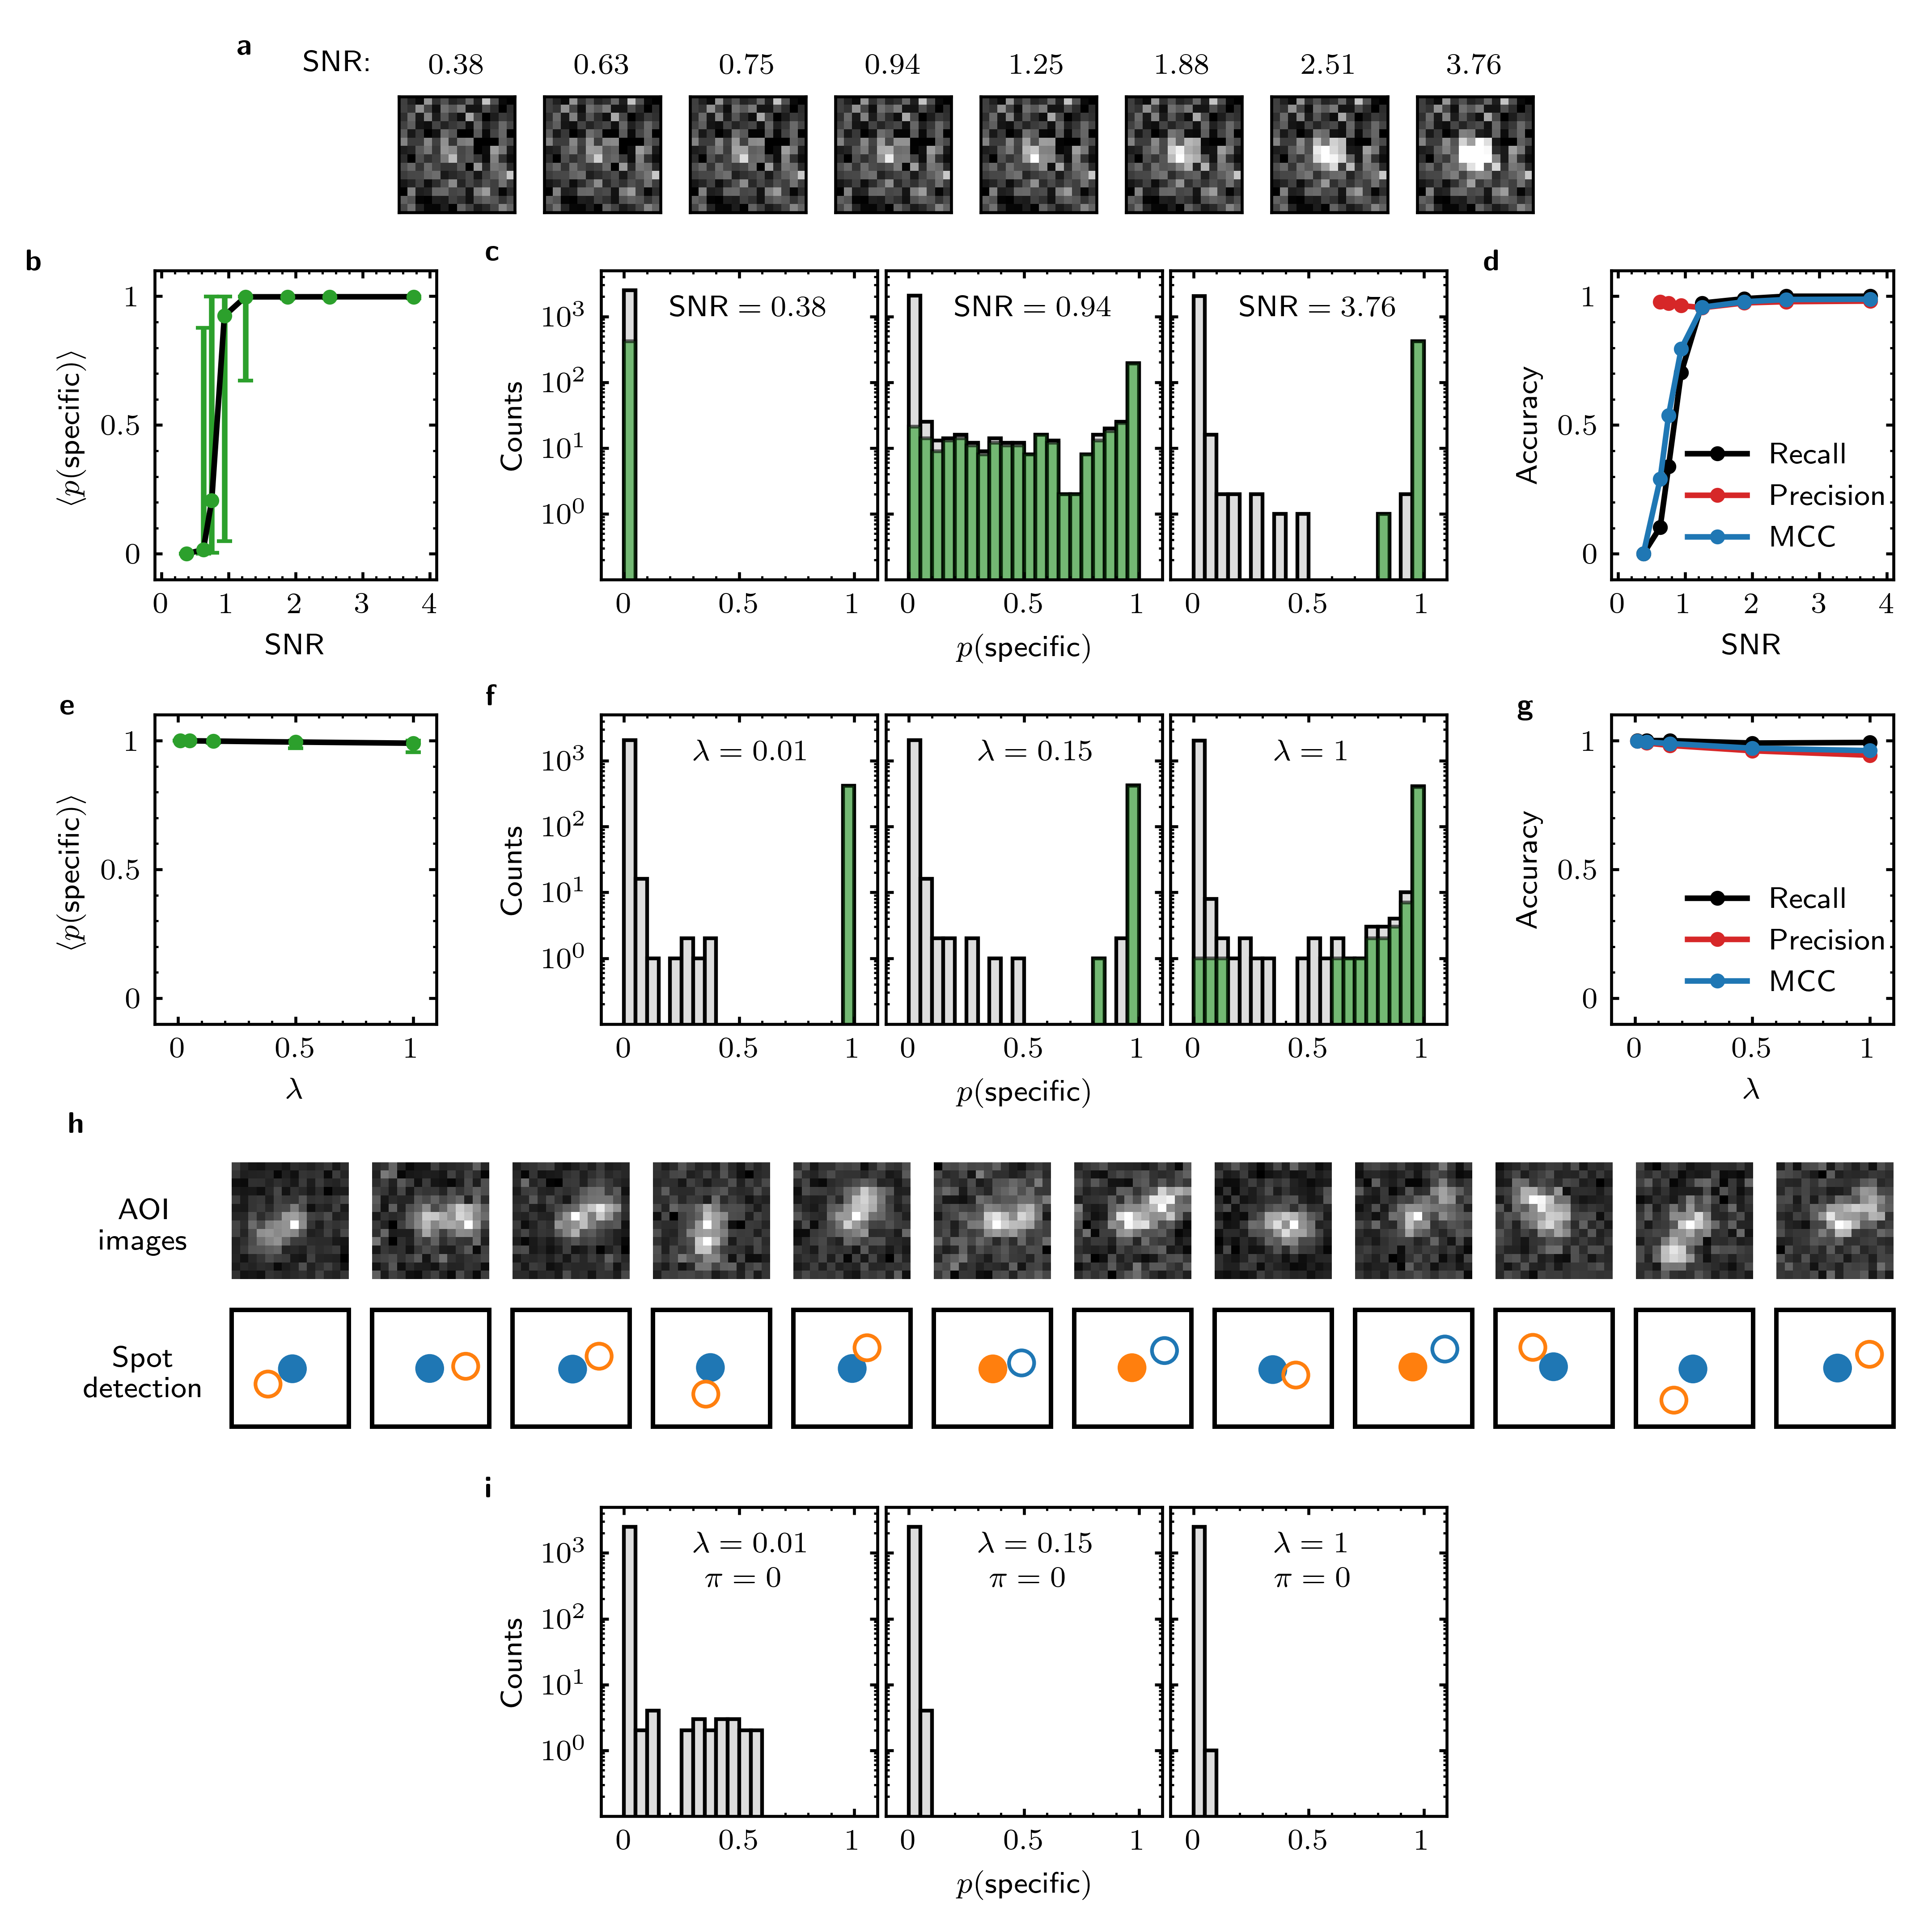
\includegraphics[width=\linewidth]{figures/figure5.png}
\caption{Performance comparison of the Bayesian method with the heuristic spot thresholding algorithm on simulated data.}
\label{fig:simulated_data}
\end{figure}

\subsection{Probabilistic modeling based on fundamental statistical analysis of data and priors}

To solve the problems with existing CoSMoS data analysis methods identified above, we have developed a new image-analysis-based approach that is accurate, objective, and built on a rigorous statistical approach to the CoSMoS image analysis problem. This TIBSD method is based on probabilistic modeling methodology. Bayesian model is a statistical model where probability is used to represent all uncertainty within the model, both for observed and hidden quantities in a system of interest. Bayes' theorem allows to perform inference on hidden variables given the observed data. The proposed first use of these methods for CoSMoS allows straightforward estimates of the uncertainty for estimated model parameters and rigorous quantitative testing of alternative image, noise, and kinetic models. “Time-independent” in the name TIBSD indicates that we ignore the time dimension of the recording -- the order of the images is arbitrary and does not affect the model, as each image is considered statistically independent of the others. We note that this time-independent method can naturally be extended into a time-dependent approach to both more accurately analyze the images and to directly obtain information about molecular kinetic mechanisms.  The proposed methods will eliminate the need for subjective image inspection and minimize the manual work required for CoSMoS data analysis.